% ============================================================
%  main.tex  --  ICEIB Conference Paper (IEEE IEEEtran format)
%  Title: An Indoor Navigation Task-Decision Agent for
%         TurtleBot3 Burger: Design and Offline Prototype Evaluation
%  Author: [Author — to be confirmed] — DIC4 Personal Assignment
%  Source group project: https://github.com/hank050392/tb3-navigation-agent
%  Compile: pdflatex main.tex  (twice for cross-references)
%           or: latexmk -pdf main.tex
% ============================================================
\documentclass[conference]{IEEEtran}

% ---- Packages ----
\usepackage{cite}
\usepackage{amsmath,amssymb,amsfonts}
\usepackage{algorithmic}
\usepackage{graphicx}
\usepackage{textcomp}
\usepackage{xcolor}
\usepackage{hyperref}
\usepackage{booktabs}
\usepackage{array}
\usepackage{url}

% ---- TikZ for architecture diagram (no external image needed) ----
\usepackage{tikz}
\usetikzlibrary{shapes.geometric, arrows.meta, positioning, fit, backgrounds}

% ---- Metadata ----
\hypersetup{
  pdftitle={An Indoor Navigation Task-Decision Agent for TurtleBot3 Burger},
  pdfauthor={DIC4 Assignment Author},
  colorlinks=true,
  linkcolor=blue,
  citecolor=blue,
  urlcolor=blue
}

% ============================================================
\begin{document}

\title{An Indoor Navigation Task-Decision Agent for TurtleBot3 Burger:\\
Design and Offline Prototype Evaluation}

% ---- Author block ----
% NOTE: English name, affiliation, and email to be confirmed by student.
% Placeholder strings are compilable; replace before final submission.
\author{
  \IEEEauthorblockN{[Author Name --- to be confirmed]\,\textsuperscript{*}}
  \IEEEauthorblockA{
    \textit{[Department --- to be confirmed]}\\
    \textit{[University --- to be confirmed]}\\
    Email: [student-email@university.edu --- to be confirmed]
  }
  \and
  \IEEEauthorblockN{(Group 7 Collaborators\,\textsuperscript{\dag})}
  \IEEEauthorblockA{
    [Names --- to be confirmed]\\
    \textit{Shared group project — hank050392/tb3-navigation-agent}
  }
}

\maketitle

% ---- Abstract ----
\begin{abstract}
Indoor mobile robots require not only path planning and obstacle avoidance, but
also accurate understanding of user-issued tasks. This paper presents the design
and offline prototype evaluation of a task-decision agent for TurtleBot3 Burger.
The proposed agent accepts Chinese-language destination commands, structures them
into validated task schemas, performs landmark whitelist verification and robot
status checks, dispatches navigation goals to the Nav2 stack, and reports results
grounded in action-server feedback. We define three system components---intent
parsing, task validation, and navigation dispatch---and implement offline contract
verification covering seven distinct outcome states: \textsc{arrived},
\textsc{clarify}, \textsc{not\_ready}, \textsc{no\_path}, \textsc{failed},
\textsc{timeout}, and \textsc{canceled}. All nine unit tests pass on the implemented
offline prototype. LLM integration, ROS~2/Nav2 connection, and physical robot
experiments remain as planned work. The paper is explicit about the boundary between
implemented offline behavior and planned integration.
\end{abstract}

\begin{IEEEkeywords}
indoor navigation, task-decision agent, TurtleBot3, ROS 2, Nav2, natural language
interface, Chinese command processing, robot task management
\end{IEEEkeywords}

% ============================================================
\section{Introduction}

TurtleBot3 Burger is a low-cost differential-drive robot widely used in robotics
education and ROS~2 research. Its standard navigation stack---Nav2 combined with
SLAM Toolbox---handles path planning and obstacle avoidance reliably in pre-mapped
indoor environments~\cite{macenski2020marathon,macenski2021slam}. However, bridging
human language to executable navigation goals introduces additional challenges:
natural language destination references may be ambiguous, robot status may be stale,
path feasibility must be confirmed before dispatch, and mission outcomes must be
reported with traceable evidence.

Existing work on language-grounded robot navigation has demonstrated that large
language models (LLMs) can parse task requests and select robot actions~\cite{yao2023react,ahn2022saycan}.
Recent studies further highlight that latency in LLM-to-ROS-2 integration remains a
practical concern~\cite{pollini2025latency}. The BARN Challenge continues to benchmark
navigation reliability in constrained environments~\cite{xiao2022barn,xiao2026barn},
demonstrating that physical execution quality cannot be inferred from language-layer
success alone.

This paper addresses the following problem: given a Chinese-language instruction from
a novice user, a registered set of named indoor locations, a pre-built occupancy map,
and a live robot status, the agent must decide whether to request clarification,
pre-empt dispatch due to robot unavailability, send a validated navigation goal, and
produce a result report grounded in the navigation action result---not in a
language-model guess.

\smallskip\noindent\textit{Attribution.} This work is a DIC4 personal assignment
reporting on the offline prototype contribution of Group~7's collaborative project
(source commit: \texttt{1c322b8}, repository: \texttt{hank050392/tb3-navigation-agent}).

The main contributions of this paper are:
\begin{enumerate}
  \item A structured task-decision architecture separating intent parsing, domain
        validation, and navigation dispatch from the underlying Nav2 stack.
  \item An offline prototype implementing landmark whitelist validation and seven
        mock outcome states, verified by nine passing unit tests.
  \item Representative test case results with actual observed JSON outputs.
  \item A comparative evaluation design (B0/B1/B2) with defined metrics and
        ablations for future full-system experiments.
\end{enumerate}

% ============================================================
\section{Related Work}

\subsection{Language Models and Robot Task Planning}

ReAct~\cite{yao2023react} demonstrates that interleaving reasoning traces and
tool-use actions improves LLM task completion on structured environments.
SayCan~\cite{ahn2022saycan} grounds robot affordances in language model outputs by
filtering actions to those physically feasible for the robot. Both approaches motivate
the design principle that language understanding should be separated from physical
execution and constrained to actions the system can actually perform.

Pollini et al.~\cite{pollini2025latency} specifically address LLM-to-ROS-2 latency,
showing that command processing delay is a practical concern for real-time robot
interaction. This motivates our decision to track separate timing components (parse
latency, dispatch latency, and feedback latency) in the planned evaluation.

\subsection{Navigation Stack and Benchmarks}

The Nav2 navigation system~\cite{macenski2020marathon} provides a behavior-tree-based
architecture for path planning, controller execution, and recovery behaviors.
SLAM Toolbox~\cite{macenski2021slam} offers efficient 2D mapping and localization
suitable for TurtleBot3 Burger. Both are integral to the planned system integration.

The BARN Challenge~\cite{xiao2022barn,xiao2026barn} and NavBench~\cite{elhariry2025navbench}
benchmark navigation reliability across classical and learned planners, establishing
that navigation success rates are environment- and configuration-dependent.

\subsection{TurtleBot3 Platform}

ROBOTIS documentation~\cite{robotis2024tb3} specifies TurtleBot3 Burger hardware:
a 2D LiDAR, two Dynamixel servos, and an onboard Raspberry Pi. Physical sensor
limitations (LiDAR blind zones, 2D-only plane detection, wheel odometry drift) are
acknowledged design factors to be measured during integration.

% ============================================================
\section{System Architecture and Method}

\subsection{Overview}

The proposed system follows a layered architecture with five modules:
(1)~Chinese Input and Intent Parser,
(2)~Task Agent and Planner,
(3)~Domain Knowledge and Validation,
(4)~Navigation Dispatch (Nav2 Adapter), and
(5)~Result Reporting.
Fig.~\ref{fig:arch} shows the complete planned architecture, distinguishing
implemented components (solid boxes) from planned integration (dashed boxes).

\begin{figure}[htbp]
\centering
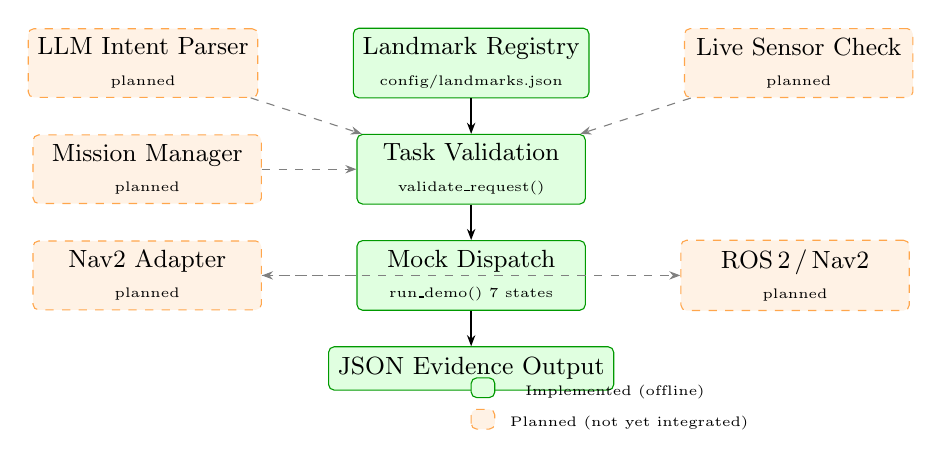
\begin{tikzpicture}[
  font=\small,
  node distance=0.45cm and 0.3cm,
  box/.style={rectangle, rounded corners=2pt, draw, minimum width=2.9cm,
              minimum height=0.55cm, align=center, fill=white},
  impl/.style={box, fill=green!12, draw=green!60!black},
  plan/.style={box, fill=orange!10, draw=orange!70, dashed},
  arr/.style={-{Stealth[length=4pt]}, thick},
  darr/.style={-{Stealth[length=4pt]}, dashed, gray}
]
  % Implemented nodes
  \node[impl] (val)  {Task Validation\\{\tiny validate\_request()}};
  \node[impl, above=of val] (lm)   {Landmark Registry\\{\tiny config/landmarks.json}};
  \node[impl, below=of val] (mock) {Mock Dispatch\\{\tiny run\_demo() 7 states}};
  \node[impl, below=of mock](evid) {JSON Evidence Output};

  % Planned nodes
  \node[plan, left=1.2cm of lm]   (llm)  {LLM Intent Parser\\{\tiny planned}};
  \node[plan, left=1.2cm of val]  (mm)   {Mission Manager\\{\tiny planned}};
  \node[plan, left=1.2cm of mock] (na)   {Nav2 Adapter\\{\tiny planned}};
  \node[plan, right=1.2cm of lm]  (sens) {Live Sensor Check\\{\tiny planned}};
  \node[plan, right=1.2cm of mock](ros)  {ROS\,2\,/\,Nav2\\{\tiny planned}};

  % Arrows implemented
  \draw[arr] (lm)   -- (val);
  \draw[arr] (val)  -- (mock);
  \draw[arr] (mock) -- (evid);

  % Arrows planned
  \draw[darr] (llm)  -- (val);
  \draw[darr] (mm)   -- (val);
  \draw[darr] (na)   -- (ros);
  \draw[darr] (sens) -- (val);
  \draw[darr] (mock) -- (na);

  % Legend
  \begin{scope}[shift={(0,-2.9)}]
    \draw[impl] (0,0) rectangle (0.3,0.25) node[right=2pt,yshift=-5pt]
      {\tiny Implemented (offline)};
    \draw[plan] (0,-0.4) rectangle (0.3,-0.15) node[right=2pt,yshift=-5pt]
      {\tiny Planned (not yet integrated)};
  \end{scope}
\end{tikzpicture}
\caption{System architecture. Solid green boxes are implemented in the offline
prototype; dashed orange boxes are planned for future integration.}
\label{fig:arch}
\end{figure}

\subsection{Task Flow}

Upon receiving Chinese-language user input, the LLM intent parser (planned) produces
a structured JSON object with fields \texttt{intent} and either \texttt{landmark\_id}
(navigate), \texttt{question} (clarify), or \texttt{reason} (reject). This object is
validated against per-intent field schemas and a landmark whitelist. If validation
fails, the task is \textsc{rejected} without navigation dispatch. The agent then checks
robot status (planned); if checks fail, \textsc{not\_ready} or \textsc{busy} is
returned. Only after all checks pass is the navigation goal sent to Nav2 (planned).
The agent monitors navigation feedback and returns \textsc{arrived}, \textsc{failed},
\textsc{timeout}, or \textsc{canceled} based on the action result.

\subsection{Task Schema}

The offline prototype validates four intent types:
\begin{itemize}
  \item \texttt{navigate}: \{``intent'': ``navigate'', ``landmark\_id'': \textit{id}\}
  \item \texttt{cancel}: \{``intent'': ``cancel''\}
  \item \texttt{clarify}: \{``intent'': ``clarify'', ``question'': \textit{str}\}
  \item \texttt{reject}: \{``intent'': ``reject'', ``reason'': \textit{str}\}
\end{itemize}
Extra fields in any request are rejected. Registered offline demo landmarks:
\texttt{desk} (experiment desk, $x$=1.0, $y$=1.0), \texttt{door\_a} (Door A, $x$=2.0, $y$=0.0),
\texttt{door\_b} (Door B, $x$=0.0, $y$=2.0). Coordinates are offline demo values only.

\subsection{Decision Algorithm}

The core algorithm (summarized from \texttt{DESIGN.md}) is:

\begin{algorithmic}[1]
\REQUIRE query $Q$, landmark registry $K$, robot status $S$
\ENSURE mission result $R$ with evidence $E$
\IF{$Q$ is explicit cancel}
  \STATE cancel active goal; \textbf{return} \textsc{canceled} (\texttt{stop\_confirmed}=false)
\ENDIF
\IF{another mission is active}
  \STATE \textbf{return} \textsc{busy}
\ENDIF
\STATE parse $Q$ into schema-constrained intent via LLM \hfill\textit{(planned)}
\IF{parsing fails or ambiguous}
  \STATE \textbf{return} \textsc{clarify}
\ENDIF
\STATE validate landmark\_id against whitelist $K$ \hfill\textit{(implemented)}
\IF{invalid}
  \STATE \textbf{return} \textsc{rejected} (no goal sent) \hfill\textit{(implemented)}
\ENDIF
\STATE check sensor freshness, localization, TF \hfill\textit{(planned)}
\IF{checks fail}
  \STATE \textbf{return} \textsc{not\_ready} with evidence
\ENDIF
\STATE check path feasibility; resolve landmark to pose \hfill\textit{(planned)}
\IF{no valid path}
  \STATE \textbf{return} \textsc{no\_path}
\ENDIF
\STATE dispatch validated goal via Nav2 adapter \hfill\textit{(planned)}
\WHILE{deadline not expired}
  \STATE monitor feedback; handle cancel, stale, result
\ENDWHILE
\STATE \textbf{return} observed terminal result with evidence $E$
\end{algorithmic}

% ============================================================
\section{Prototype Implementation}

\subsection{Implementation Scope}

The offline prototype is implemented in Python~3.10+ using only the standard library.
No API keys, ROS~2, Gazebo, or third-party Python packages are required. Entry point:
\texttt{src/agent\_demo.py}; validation logic: \texttt{validate\_request()};
scenario branching: \texttt{run\_demo()}.

\subsection{Executed Test Scenarios}

Table~\ref{tab:results} summarizes the actual observed outputs for all demo scenarios
(source commit \texttt{1c322b8}). All outputs include \texttt{demo\_only: true} and
\texttt{navigation\_backend: "mock"}.

\begin{table}[htbp]
\caption{Offline Demo Scenario Results (Commit 1c322b8, All Observed)}
\label{tab:results}
\centering
\renewcommand{\arraystretch}{1.1}
\begin{tabular}{@{}p{1.8cm}p{1.4cm}p{0.8cm}@{}}
\toprule
\textbf{Scenario} & \textbf{Status} & \textbf{goal\_sent} \\
\midrule
Normal navigate (ready)  & ARRIVED    & true  \\
Ambiguous (clarify)      & CLARIFY    & false \\
Stale sensor (stale)     & NOT\_READY & false \\
Path blocked (blocked)   & NO\_PATH   & false \\
Nav failed (failed)      & FAILED     & true  \\
Nav timeout (timeout)    & TIMEOUT    & true  \\
Robot busy (busy)        & BUSY       & false \\
Cancel (busy)            & CANCELED   & false \\
Unknown landmark         & REJECTED   & false \\
\bottomrule
\end{tabular}
\end{table}

\subsection{Unit Test Results}

\noindent Command: \texttt{python3 -m unittest discover -s tests -v}

\noindent Result: \textbf{Ran 9 tests in 0.001s --- OK} (all pass)

The test suite verifies: valid goal returns \textsc{arrived} with
\texttt{demo\_only=true}; unknown landmark rejected without dispatch; extra schema
fields rejected; bad schema types rejected; stale/blocked/busy do not dispatch;
clarify does not dispatch; \textsc{failed} and \textsc{timeout} are not
\textsc{arrived}; cancel sets \texttt{stop\_confirmed=false}; empty question rejected.

% ============================================================
\section{Evaluation and Results}

\subsection{Offline Contract Evaluation (Completed)}

The offline prototype satisfies all contract requirements verified by the unit test
suite. These tests confirm schema enforcement, whitelist exclusivity, no dispatch on
invalid or adverse status, correct cancel semantics, and evidence fields in all
outputs. These tests do not evaluate LLM accuracy, navigation success rates, or
physical robot behavior.

\subsection{Planned Comparative Evaluation}

Three navigation interface methods are designed for comparison:
\begin{itemize}
  \item \textbf{B0:} Fixed landmark menu + Nav2 (baseline; no natural language).
  \item \textbf{B1:} LLM-direct parsing + schema/whitelist + Nav2.
  \item \textbf{B2:} Full agent (B1 + clarification + status check + evidence).
\end{itemize}

Planned dataset: 60 Chinese commands (clear, ambiguous, unknown, cancel, compound,
conflicting; 20 dev / 40 test). Planned scenarios: open space, narrow corridor, added
obstacle, abnormal status. Planned runs: 40 per method (simulation), 36 physical.

Planned metrics: processing accuracy, improper dispatch rate, task completion rate,
navigation success rate, report accuracy, latency (p50/p95), path length, and
collision/clearance. All are defined with numerator/denominator and Wilson 95\%
confidence intervals. Table~\ref{tab:plan} summarizes the evaluation plan.

\begin{table}[htbp]
\caption{Planned Evaluation Design --- No Results Yet}
\label{tab:plan}
\centering
\renewcommand{\arraystretch}{1.1}
\begin{tabular}{@{}p{2.4cm}p{1.0cm}p{1.5cm}@{}}
\toprule
\textbf{Metric} & \textbf{Methods} & \textbf{Status} \\
\midrule
Processing accuracy   & B1, B2    & Not executed \\
Improper dispatch     & B1, B2    & Not executed \\
Task completion       & B0,B1,B2  & Not executed \\
Navigation success    & B0,B1,B2  & Not executed \\
Report accuracy       & B1, B2    & Not executed \\
Latency p50/p95       & B1, B2    & Not executed \\
\bottomrule
\end{tabular}
\end{table}

\noindent\textbf{No numerical navigation or LLM results exist} at the time of this
paper submission. \texttt{data/results\_template.csv} provides column headers for
future result recording.

% ============================================================
\section{Limitations and Future Work}

Current limitations of the prototype:
(1) No LLM integration: Chinese natural language is not yet parsed; the prototype
    accepts pre-structured JSON only.
(2) No ROS~2/Nav2 integration: navigation outcomes are mocked; no physical robot is
    controlled.
(3) No live sensor checks: stale/busy/blocked states are injected via CLI scenario
    flag, not read from real robot sensors.
(4) Single flat indoor environment: one TurtleBot3 Burger, one pre-built 2D map,
    human-named registered destinations only.
(5) No dynamic obstacle modeling beyond Nav2's built-in recovery behaviors.

Planned future work includes connecting an LLM with structured output, implementing
the mission manager and Nav2 adapter, executing B0/B1/B2 comparative experiments
with real sensor and navigation data, and extending to multi-destination tasks.

% ============================================================
\section{Conclusion}

This paper presents the design and offline prototype evaluation of a Chinese-language
task-decision agent for TurtleBot3 Burger indoor navigation. The agent architecture
separates intent parsing, landmark validation, and navigation dispatch into verifiable
layers. The offline prototype implements seven outcome states, three registered
landmarks, and schema-enforced validation, confirmed by nine passing unit tests with
all scenarios producing expected outputs. No physical robot motion occurs.

The paper explicitly distinguishes implemented offline behavior---schema validation,
whitelist rejection, mock outcome branching---from planned integration: LLM parsing,
live sensor checks, and ROS~2/Nav2 dispatch. No navigation success rates, LLM accuracy
figures, or physical timing measurements are reported, as none have been measured.

This work contributes a structured evaluation design and evidence-grounded reporting
framework for future full-system experiments comparing fixed menu, direct LLM, and
full agent navigation interfaces.

% ============================================================
\section*{Acknowledgment}

The offline prototype, system design, and project documentation were developed
collaboratively by Group~7 (DIC course). This individual assignment paper is based
on the shared group project repository
(\url{https://github.com/hank050392/tb3-navigation-agent}).

% ============================================================
\bibliographystyle{IEEEtran}
\bibliography{references}

\end{document}
